\subsection{The CML Metamodel (Abstract Syntax)}\label{subsec:metamodel}

In the article \emph{UML and OCL in Conceptual Modeling}, 
Gogolla \cite{gogolla} shows, by mapping the UML \cite{uml} metamodel to the ER \cite{er} metamodel,
how UML models (augmented by OCL \cite{ocl} constraints) can be used to specify conceptual models.
Also, Wazlawick \cite{wazlawick} systematically prescribes in his book a method for conceptual modeling using UML and OCL. 

Since one key CML goal is enabling the specification of conceptual models
(such as those specified by ER models and UML/OCL models),
in order to present the key elements of the CML metamodel,
a similar approach to Gogolla's is used to map the CML metamodel to the ER metamodel,
and to the UML/OCL metamodel.

The EMOF \cite{mof} model presented by figure \ref{fig:metamodel} is a simplified version of the CML metamodel:

\begin{figure}
\centering
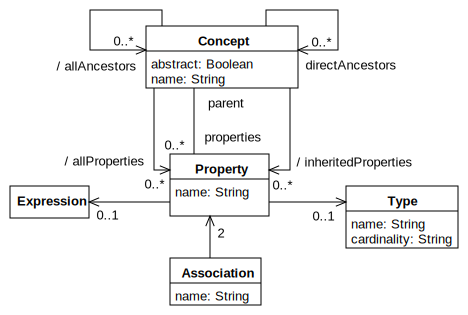
\includegraphics[width=0.8\textwidth]{language/diagram-metamodel}
\caption{This class diagram renders the EMOF \cite{mof} model defining the CML metamodel.}
\label{fig:metamodel}
\end{figure}

In CML metamodel shown in figure \ref{fig:metamodel},
a \emph{Concept} is composed of zero-or-more \emph{Property} instances.
Each \emph{Property} may have a \emph{Type} and an \emph{Expression}.
If two \emph{Property} instances represent the same bidirectional association,
there must be an \emph{Association} instance that binds them.
Unidirectional associations are only represented by the \emph{Property} instance (representing the association role)
that enables the navigation from the source \emph{Concept} instance to the target one (which is represented by the property's \emph{Type}.)

Next, there is a description for the key metamodel elements.

\subsubsection{Concept.}

According to Wazlawick \cite{wazlawick},
a concept represents complex information that has a coherent meaning in the domain.
They aggregate attributes and cannot be described as primitive values.
They may also be associated with other concepts.
On the ER metamodel, it is known as \emph{entity};
on the UML metamodel, as \emph{class}.

\subsubsection{Property.}

May hold values of primitive types, in which case they represent an attribute on the \emph{ER} and \emph{UML} metamodels;
or may hold references (or collections of references) linking to instances of other concepts.
On the ER metamodel,
a set of all references linking one entity instance to another is known as a \emph{relationship};
on the UML metamodel, it is known as a \emph{unidirectional association}.

\subsubsection{Association.}

Unlike the ER and UML metamodels, in the CML metamodel, only bidirectional associations are represented with the Association class. Using UML terminology, they bind the reference (non-primitive) properties (of the same, or different concepts),
so that the association links are accessible from each association end participating in the association.
It directly represents in the CML metamodel what normally requires additional implementation in programming languages.
It is inspired\footnote{The syntax used in CML resembles the syntax of a \emph{struct} in C \cite{clang}, while Cardoso \cite{cardoso} uses a verbose syntax. Also, unlike CML, Cardoso does \emph{not} bind properties that represent each association end; instead, associations -- unidirectional or bidirectional -- are declared independently of class properties.} on the work of Cardoso \cite{cardoso}, which extends the C\# language to represent bidirectional associations.

TODO: Referencia a BALZER; GROSS; EUGSTER, 2007: interposition of elements.

\subsubsection{Type.} They may be primitive types (such as Boolean, String, Decimal, and Regex), references to concept instances, or still collections of concepts, depending on the \emph{cardinality} property. They may also be optional, meaning their value may or may not have been set; also defined by the \emph{cardinality} property.
